% Options for packages loaded elsewhere
\PassOptionsToPackage{unicode}{hyperref}
\PassOptionsToPackage{hyphens}{url}
\PassOptionsToPackage{dvipsnames,svgnames,x11names}{xcolor}
%
\documentclass[
  letterpaper,
  DIV=11,
  numbers=noendperiod]{scrartcl}

\usepackage{amsmath,amssymb}
\usepackage{iftex}
\ifPDFTeX
  \usepackage[T1]{fontenc}
  \usepackage[utf8]{inputenc}
  \usepackage{textcomp} % provide euro and other symbols
\else % if luatex or xetex
  \usepackage{unicode-math}
  \defaultfontfeatures{Scale=MatchLowercase}
  \defaultfontfeatures[\rmfamily]{Ligatures=TeX,Scale=1}
\fi
\usepackage{lmodern}
\ifPDFTeX\else  
    % xetex/luatex font selection
\fi
% Use upquote if available, for straight quotes in verbatim environments
\IfFileExists{upquote.sty}{\usepackage{upquote}}{}
\IfFileExists{microtype.sty}{% use microtype if available
  \usepackage[]{microtype}
  \UseMicrotypeSet[protrusion]{basicmath} % disable protrusion for tt fonts
}{}
\makeatletter
\@ifundefined{KOMAClassName}{% if non-KOMA class
  \IfFileExists{parskip.sty}{%
    \usepackage{parskip}
  }{% else
    \setlength{\parindent}{0pt}
    \setlength{\parskip}{6pt plus 2pt minus 1pt}}
}{% if KOMA class
  \KOMAoptions{parskip=half}}
\makeatother
\usepackage{xcolor}
\setlength{\emergencystretch}{3em} % prevent overfull lines
\setcounter{secnumdepth}{-\maxdimen} % remove section numbering
% Make \paragraph and \subparagraph free-standing
\ifx\paragraph\undefined\else
  \let\oldparagraph\paragraph
  \renewcommand{\paragraph}[1]{\oldparagraph{#1}\mbox{}}
\fi
\ifx\subparagraph\undefined\else
  \let\oldsubparagraph\subparagraph
  \renewcommand{\subparagraph}[1]{\oldsubparagraph{#1}\mbox{}}
\fi

\usepackage{color}
\usepackage{fancyvrb}
\newcommand{\VerbBar}{|}
\newcommand{\VERB}{\Verb[commandchars=\\\{\}]}
\DefineVerbatimEnvironment{Highlighting}{Verbatim}{commandchars=\\\{\}}
% Add ',fontsize=\small' for more characters per line
\usepackage{framed}
\definecolor{shadecolor}{RGB}{241,243,245}
\newenvironment{Shaded}{\begin{snugshade}}{\end{snugshade}}
\newcommand{\AlertTok}[1]{\textcolor[rgb]{0.68,0.00,0.00}{#1}}
\newcommand{\AnnotationTok}[1]{\textcolor[rgb]{0.37,0.37,0.37}{#1}}
\newcommand{\AttributeTok}[1]{\textcolor[rgb]{0.40,0.45,0.13}{#1}}
\newcommand{\BaseNTok}[1]{\textcolor[rgb]{0.68,0.00,0.00}{#1}}
\newcommand{\BuiltInTok}[1]{\textcolor[rgb]{0.00,0.23,0.31}{#1}}
\newcommand{\CharTok}[1]{\textcolor[rgb]{0.13,0.47,0.30}{#1}}
\newcommand{\CommentTok}[1]{\textcolor[rgb]{0.37,0.37,0.37}{#1}}
\newcommand{\CommentVarTok}[1]{\textcolor[rgb]{0.37,0.37,0.37}{\textit{#1}}}
\newcommand{\ConstantTok}[1]{\textcolor[rgb]{0.56,0.35,0.01}{#1}}
\newcommand{\ControlFlowTok}[1]{\textcolor[rgb]{0.00,0.23,0.31}{#1}}
\newcommand{\DataTypeTok}[1]{\textcolor[rgb]{0.68,0.00,0.00}{#1}}
\newcommand{\DecValTok}[1]{\textcolor[rgb]{0.68,0.00,0.00}{#1}}
\newcommand{\DocumentationTok}[1]{\textcolor[rgb]{0.37,0.37,0.37}{\textit{#1}}}
\newcommand{\ErrorTok}[1]{\textcolor[rgb]{0.68,0.00,0.00}{#1}}
\newcommand{\ExtensionTok}[1]{\textcolor[rgb]{0.00,0.23,0.31}{#1}}
\newcommand{\FloatTok}[1]{\textcolor[rgb]{0.68,0.00,0.00}{#1}}
\newcommand{\FunctionTok}[1]{\textcolor[rgb]{0.28,0.35,0.67}{#1}}
\newcommand{\ImportTok}[1]{\textcolor[rgb]{0.00,0.46,0.62}{#1}}
\newcommand{\InformationTok}[1]{\textcolor[rgb]{0.37,0.37,0.37}{#1}}
\newcommand{\KeywordTok}[1]{\textcolor[rgb]{0.00,0.23,0.31}{#1}}
\newcommand{\NormalTok}[1]{\textcolor[rgb]{0.00,0.23,0.31}{#1}}
\newcommand{\OperatorTok}[1]{\textcolor[rgb]{0.37,0.37,0.37}{#1}}
\newcommand{\OtherTok}[1]{\textcolor[rgb]{0.00,0.23,0.31}{#1}}
\newcommand{\PreprocessorTok}[1]{\textcolor[rgb]{0.68,0.00,0.00}{#1}}
\newcommand{\RegionMarkerTok}[1]{\textcolor[rgb]{0.00,0.23,0.31}{#1}}
\newcommand{\SpecialCharTok}[1]{\textcolor[rgb]{0.37,0.37,0.37}{#1}}
\newcommand{\SpecialStringTok}[1]{\textcolor[rgb]{0.13,0.47,0.30}{#1}}
\newcommand{\StringTok}[1]{\textcolor[rgb]{0.13,0.47,0.30}{#1}}
\newcommand{\VariableTok}[1]{\textcolor[rgb]{0.07,0.07,0.07}{#1}}
\newcommand{\VerbatimStringTok}[1]{\textcolor[rgb]{0.13,0.47,0.30}{#1}}
\newcommand{\WarningTok}[1]{\textcolor[rgb]{0.37,0.37,0.37}{\textit{#1}}}

\providecommand{\tightlist}{%
  \setlength{\itemsep}{0pt}\setlength{\parskip}{0pt}}\usepackage{longtable,booktabs,array}
\usepackage{calc} % for calculating minipage widths
% Correct order of tables after \paragraph or \subparagraph
\usepackage{etoolbox}
\makeatletter
\patchcmd\longtable{\par}{\if@noskipsec\mbox{}\fi\par}{}{}
\makeatother
% Allow footnotes in longtable head/foot
\IfFileExists{footnotehyper.sty}{\usepackage{footnotehyper}}{\usepackage{footnote}}
\makesavenoteenv{longtable}
\usepackage{graphicx}
\makeatletter
\def\maxwidth{\ifdim\Gin@nat@width>\linewidth\linewidth\else\Gin@nat@width\fi}
\def\maxheight{\ifdim\Gin@nat@height>\textheight\textheight\else\Gin@nat@height\fi}
\makeatother
% Scale images if necessary, so that they will not overflow the page
% margins by default, and it is still possible to overwrite the defaults
% using explicit options in \includegraphics[width, height, ...]{}
\setkeys{Gin}{width=\maxwidth,height=\maxheight,keepaspectratio}
% Set default figure placement to htbp
\makeatletter
\def\fps@figure{htbp}
\makeatother

\KOMAoption{captions}{tableheading}
\makeatletter
\@ifpackageloaded{tcolorbox}{}{\usepackage[skins,breakable]{tcolorbox}}
\@ifpackageloaded{fontawesome5}{}{\usepackage{fontawesome5}}
\definecolor{quarto-callout-color}{HTML}{909090}
\definecolor{quarto-callout-note-color}{HTML}{0758E5}
\definecolor{quarto-callout-important-color}{HTML}{CC1914}
\definecolor{quarto-callout-warning-color}{HTML}{EB9113}
\definecolor{quarto-callout-tip-color}{HTML}{00A047}
\definecolor{quarto-callout-caution-color}{HTML}{FC5300}
\definecolor{quarto-callout-color-frame}{HTML}{acacac}
\definecolor{quarto-callout-note-color-frame}{HTML}{4582ec}
\definecolor{quarto-callout-important-color-frame}{HTML}{d9534f}
\definecolor{quarto-callout-warning-color-frame}{HTML}{f0ad4e}
\definecolor{quarto-callout-tip-color-frame}{HTML}{02b875}
\definecolor{quarto-callout-caution-color-frame}{HTML}{fd7e14}
\makeatother
\makeatletter
\makeatother
\makeatletter
\makeatother
\makeatletter
\@ifpackageloaded{caption}{}{\usepackage{caption}}
\AtBeginDocument{%
\ifdefined\contentsname
  \renewcommand*\contentsname{Table of contents}
\else
  \newcommand\contentsname{Table of contents}
\fi
\ifdefined\listfigurename
  \renewcommand*\listfigurename{List of Figures}
\else
  \newcommand\listfigurename{List of Figures}
\fi
\ifdefined\listtablename
  \renewcommand*\listtablename{List of Tables}
\else
  \newcommand\listtablename{List of Tables}
\fi
\ifdefined\figurename
  \renewcommand*\figurename{Figure}
\else
  \newcommand\figurename{Figure}
\fi
\ifdefined\tablename
  \renewcommand*\tablename{Table}
\else
  \newcommand\tablename{Table}
\fi
}
\@ifpackageloaded{float}{}{\usepackage{float}}
\floatstyle{ruled}
\@ifundefined{c@chapter}{\newfloat{codelisting}{h}{lop}}{\newfloat{codelisting}{h}{lop}[chapter]}
\floatname{codelisting}{Listing}
\newcommand*\listoflistings{\listof{codelisting}{List of Listings}}
\makeatother
\makeatletter
\@ifpackageloaded{caption}{}{\usepackage{caption}}
\@ifpackageloaded{subcaption}{}{\usepackage{subcaption}}
\makeatother
\makeatletter
\@ifpackageloaded{tcolorbox}{}{\usepackage[skins,breakable]{tcolorbox}}
\makeatother
\makeatletter
\@ifundefined{shadecolor}{\definecolor{shadecolor}{rgb}{.97, .97, .97}}
\makeatother
\makeatletter
\makeatother
\makeatletter
\makeatother
\makeatletter
\@ifpackageloaded{tikz}{}{\usepackage{tikz}}
\makeatother
        \newcommand*\circled[1]{\tikz[baseline=(char.base)]{
          \node[shape=circle,draw,inner sep=1pt] (char) {{\scriptsize#1}};}}  
                  
\ifLuaTeX
  \usepackage{selnolig}  % disable illegal ligatures
\fi
\IfFileExists{bookmark.sty}{\usepackage{bookmark}}{\usepackage{hyperref}}
\IfFileExists{xurl.sty}{\usepackage{xurl}}{} % add URL line breaks if available
\urlstyle{same} % disable monospaced font for URLs
\hypersetup{
  pdftitle={filter, select, arrange, slice, mutate},
  pdfauthor={Emily Malcolm-White},
  colorlinks=true,
  linkcolor={blue},
  filecolor={Maroon},
  citecolor={Blue},
  urlcolor={Blue},
  pdfcreator={LaTeX via pandoc}}

\title{filter, select, arrange, slice, mutate}
\author{Emily Malcolm-White}
\date{}

\begin{document}
\maketitle
\ifdefined\Shaded\renewenvironment{Shaded}{\begin{tcolorbox}[breakable, boxrule=0pt, interior hidden, frame hidden, enhanced, sharp corners, borderline west={3pt}{0pt}{shadecolor}]}{\end{tcolorbox}}\fi

\begin{tcolorbox}[enhanced jigsaw, leftrule=.75mm, breakable, bottomrule=.15mm, colback=white, colframe=quarto-callout-important-color-frame, toptitle=1mm, opacitybacktitle=0.6, toprule=.15mm, colbacktitle=quarto-callout-important-color!10!white, rightrule=.15mm, coltitle=black, bottomtitle=1mm, titlerule=0mm, opacityback=0, title=\textcolor{quarto-callout-important-color}{\faExclamation}\hspace{0.5em}{Downloads}, arc=.35mm, left=2mm]

\begin{itemize}
\tightlist
\item
  \href{B_wrangling.qmd}{📖 Notes .qmd}
\item
  \href{B_wrangling_notes.qmd}{📝️ Notes Template .qmd}
\item
  \href{B_wrangling_homework.qmd}{📚 Homework .qmd}
\end{itemize}

\end{tcolorbox}

\hypertarget{installing-and-using-packages}{%
\section{Installing and Using
Packages}\label{installing-and-using-packages}}

Sometimes everything we need (data, functions, etc) are not available in
base R. In R, expert users will package up useful things like data and
functions into packages that be download and used.

First, you need to download the package from the right hand menu
--\textgreater{} You only need to do this once.

In each new .qmd document, you need to call any packages you want to use
but adding the code \texttt{library(packagename)} inside an R chunk.

For example, in this class we will use the \texttt{tidyverse} package a
lot.

\hypertarget{annotated-cell-1}{%
\label{annotated-cell-1}}%
\begin{Shaded}
\begin{Highlighting}[]
\FunctionTok{library}\NormalTok{(tidyverse) }\CommentTok{\#\textless{}1\textgreater{}}
\end{Highlighting}
\end{Shaded}

\begin{description}
\tightlist
\item[\circled{1}]
Loads the \texttt{tidyverse} package
\end{description}

There are actually many commonly used packages wrapped up inside one
\texttt{tidyverse} package.

\begin{figure}

{\centering 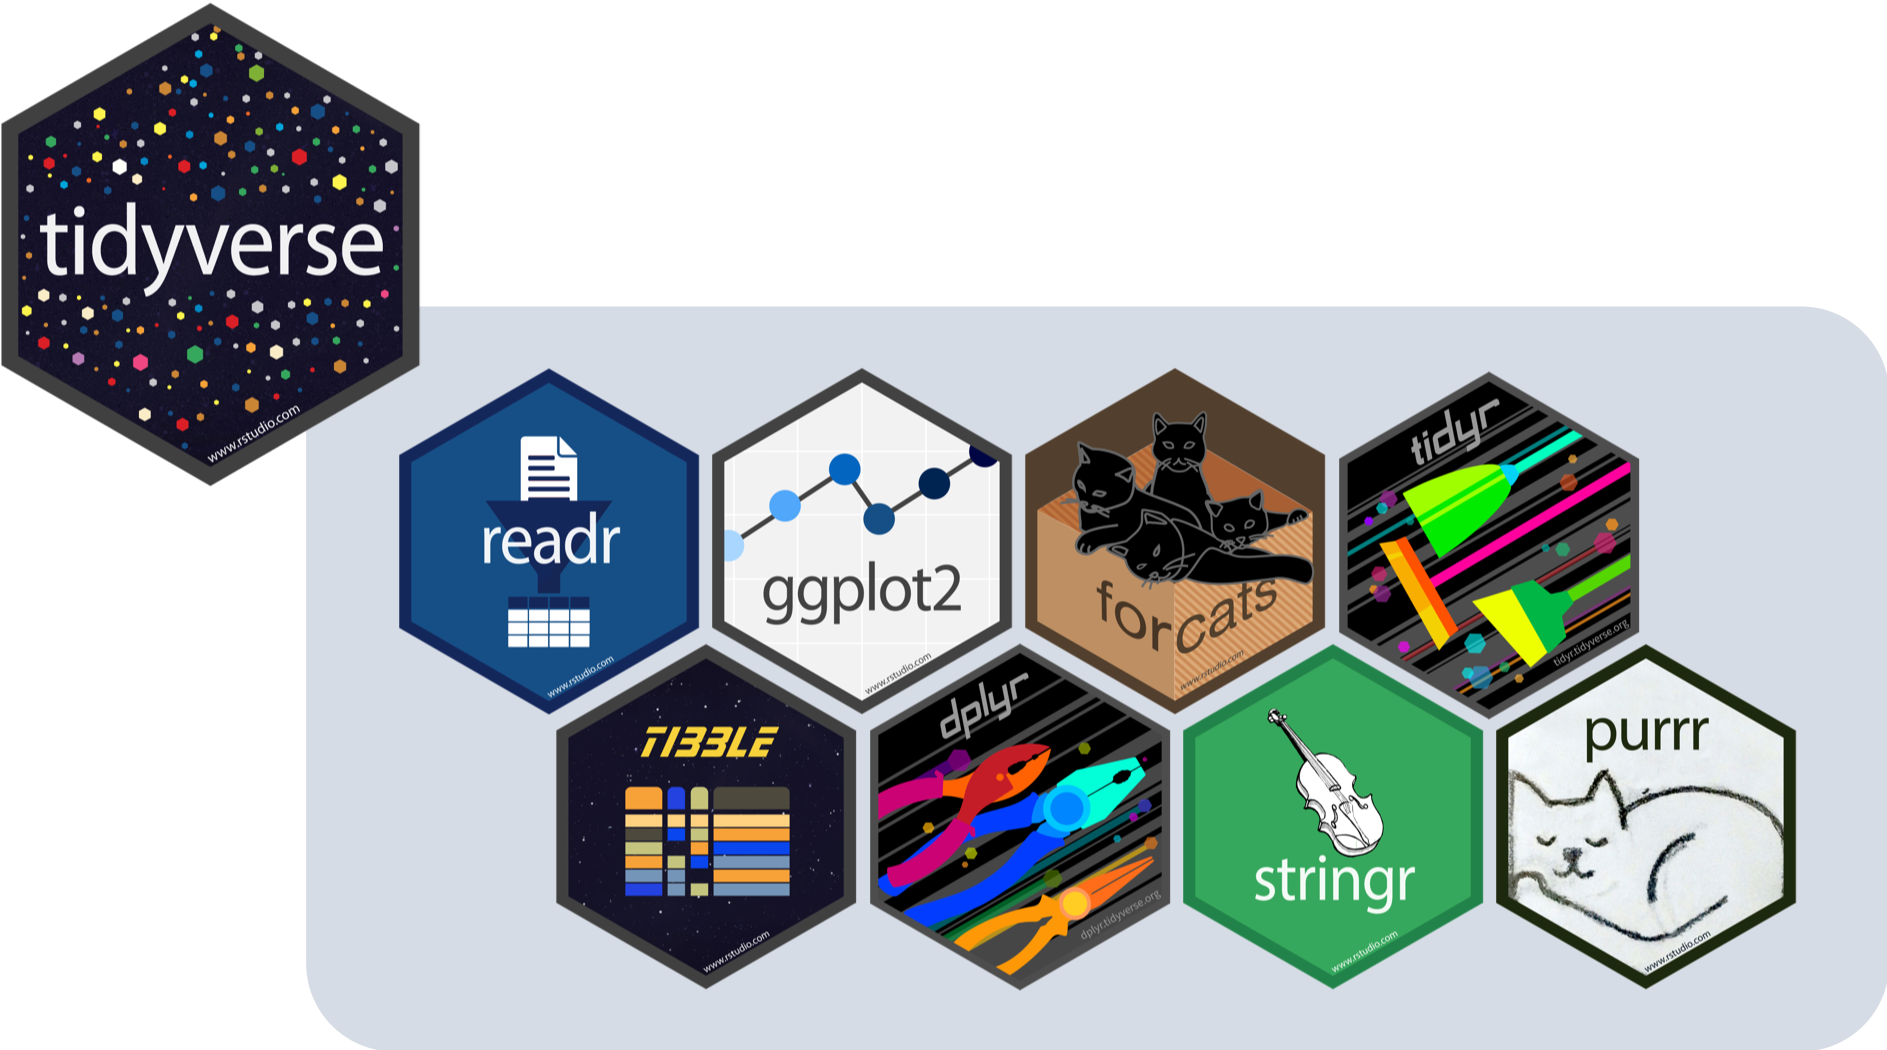
\includegraphics{images/tidyverse_packages.png}

}

\caption{Credit: https://uopsych-r-bootcamp-2020.netlify.app/}

\end{figure}

Today we are specifically going to be talking about the package
\texttt{dplyr} which is useful to manipulating data sets.

\hypertarget{can_lang-dataset}{%
\section{\texorpdfstring{\texttt{can\_lang}
dataset}{can\_lang dataset}}\label{can_lang-dataset}}

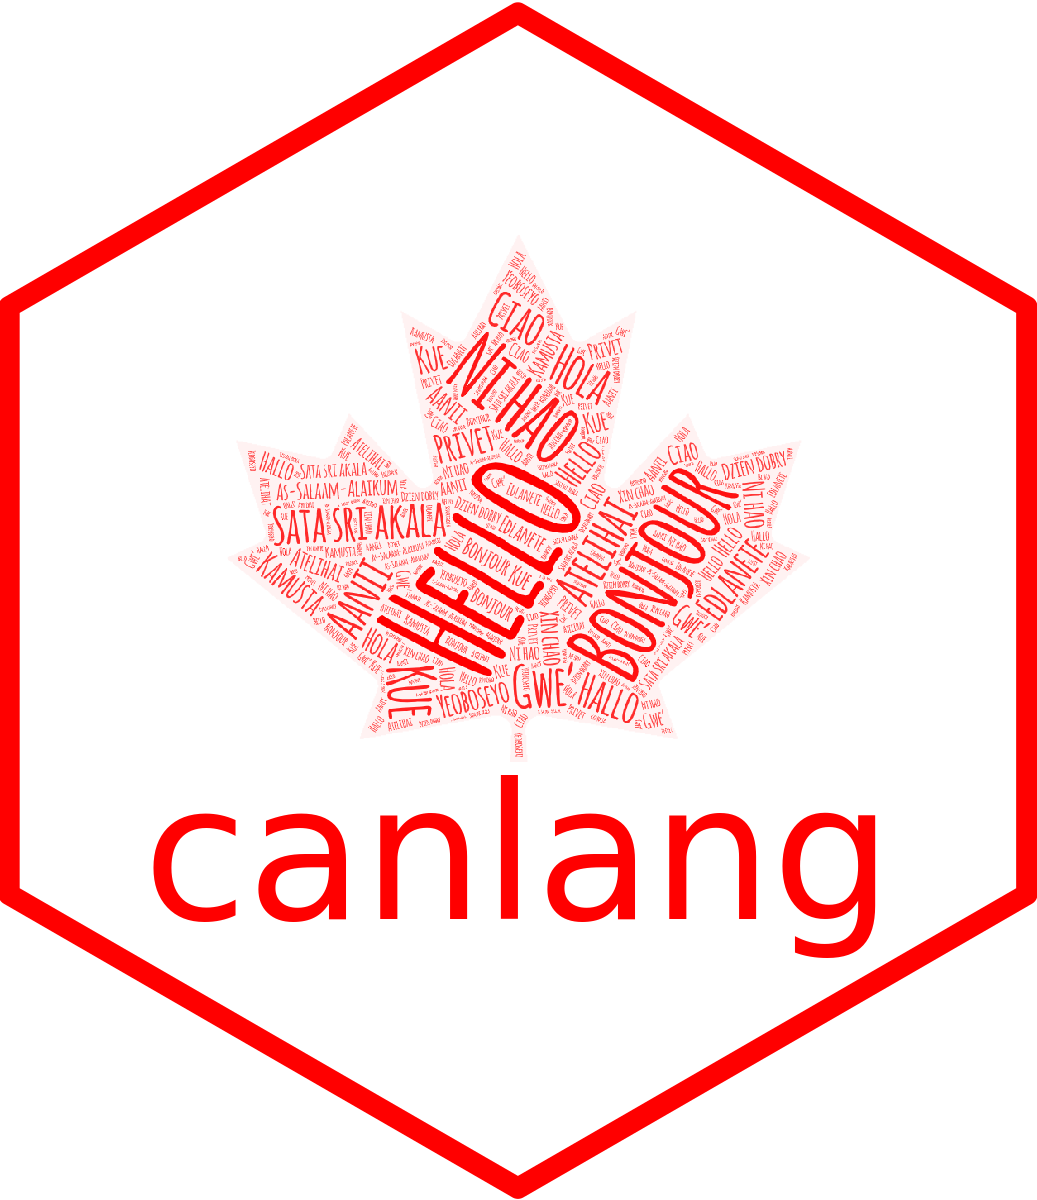
\includegraphics[width=0.3\textwidth,height=\textheight]{118_B_wrangling_files/mediabag/hex-canlang.png}

In this class, we are going to be working with a dataset relating to the
languages spoken at home by Canadian residents. Many Indigenous peoples
exist in Canada with their own languages and cultures. Sadly,
colonization has led to the loss of many of these languages. This data
is a subset of data collected during the 2016 census.

\hypertarget{importing-data}{%
\section{Importing Data}\label{importing-data}}

\textbf{What is a .csv file?}

\begin{itemize}
\tightlist
\item
  It's plain text file that stores data
\item
  Each value is seperated by a comma (,) - hence the name ``\emph{c}omma
  \emph{s}eperated \emph{v}alues''
\item
  It's readable with tools like Excel, Good Sheets, R, and more.
\end{itemize}

\textbf{How do we import it into R?} Use \texttt{read.csv()}! Note that
your data file (\texttt{.csv}) needs to be saved in the same folder as
your notes template document (\texttt{.qmd}).

\hypertarget{annotated-cell-2}{%
\label{annotated-cell-2}}%
\begin{Shaded}
\begin{Highlighting}[]
\NormalTok{can\_lang }\OtherTok{\textless{}{-}} \FunctionTok{read.csv}\NormalTok{(}\StringTok{"data/can\_lang.csv"}\NormalTok{) }\CommentTok{\#\textless{}1\textgreater{}}
\end{Highlighting}
\end{Shaded}

\begin{description}
\tightlist
\item[\circled{1}]
Takes the \texttt{can\_lang.csv} file (located in the same folder as
your .qmd file), reads it into R, and saves it as the dataset
\texttt{can\_lang}
\end{description}

Alternatively, you can download it directly from the internet. Github
user \texttt{ttimbers} hosts this file to share with the public at the
link:
\url{https://raw.githubusercontent.com/ttimbers/canlang/master/inst/extdata/can_lang.csv}

\hypertarget{annotated-cell-3}{%
\label{annotated-cell-3}}%
\begin{Shaded}
\begin{Highlighting}[]
\NormalTok{can\_lang }\OtherTok{\textless{}{-}} \FunctionTok{read.csv}\NormalTok{(}\StringTok{"https://raw.githubusercontent.com/ttimbers/canlang/master/inst/extdata/can\_lang.csv"}\NormalTok{) }\CommentTok{\#\textless{}1\textgreater{}}
\end{Highlighting}
\end{Shaded}

\begin{description}
\tightlist
\item[\circled{1}]
Takes the dataset located at the given url, reads it into R, and saves
it as the dataset \texttt{can\_lang}
\end{description}

Let's take a look at this data for a minute to see what information has
been recorded. In the environment in the top left, if you click on the
word \texttt{can\_lang} (not the blue play button, the word itself) it
will open the object so you can see what is saved inside. Alternatively
you can use the \texttt{head()} function to display just the first few
rows of the dataset.

\begin{Shaded}
\begin{Highlighting}[]
\FunctionTok{head}\NormalTok{(can\_lang)}
\end{Highlighting}
\end{Shaded}

\begin{verbatim}
                                 category                       language
1                    Aboriginal languages   Aboriginal languages, n.o.s.
2 Non-Official & Non-Aboriginal languages                      Afrikaans
3 Non-Official & Non-Aboriginal languages Afro-Asiatic languages, n.i.e.
4 Non-Official & Non-Aboriginal languages                     Akan (Twi)
5 Non-Official & Non-Aboriginal languages                       Albanian
6                    Aboriginal languages   Algonquian languages, n.i.e.
  mother_tongue most_at_home most_at_work lang_known
1           590          235           30        665
2         10260         4785           85      23415
3          1150          445           10       2775
4         13460         5985           25      22150
5         26895        13135          345      31930
6            45           10            0        120
\end{verbatim}

\hypertarget{filter}{%
\section{\texorpdfstring{\texttt{filter}}{filter}}\label{filter}}

We can use the \texttt{filter} function to extract \textbf{\emph{rows}}
from the data that have a particular characteristic.

\begin{figure}

{\centering 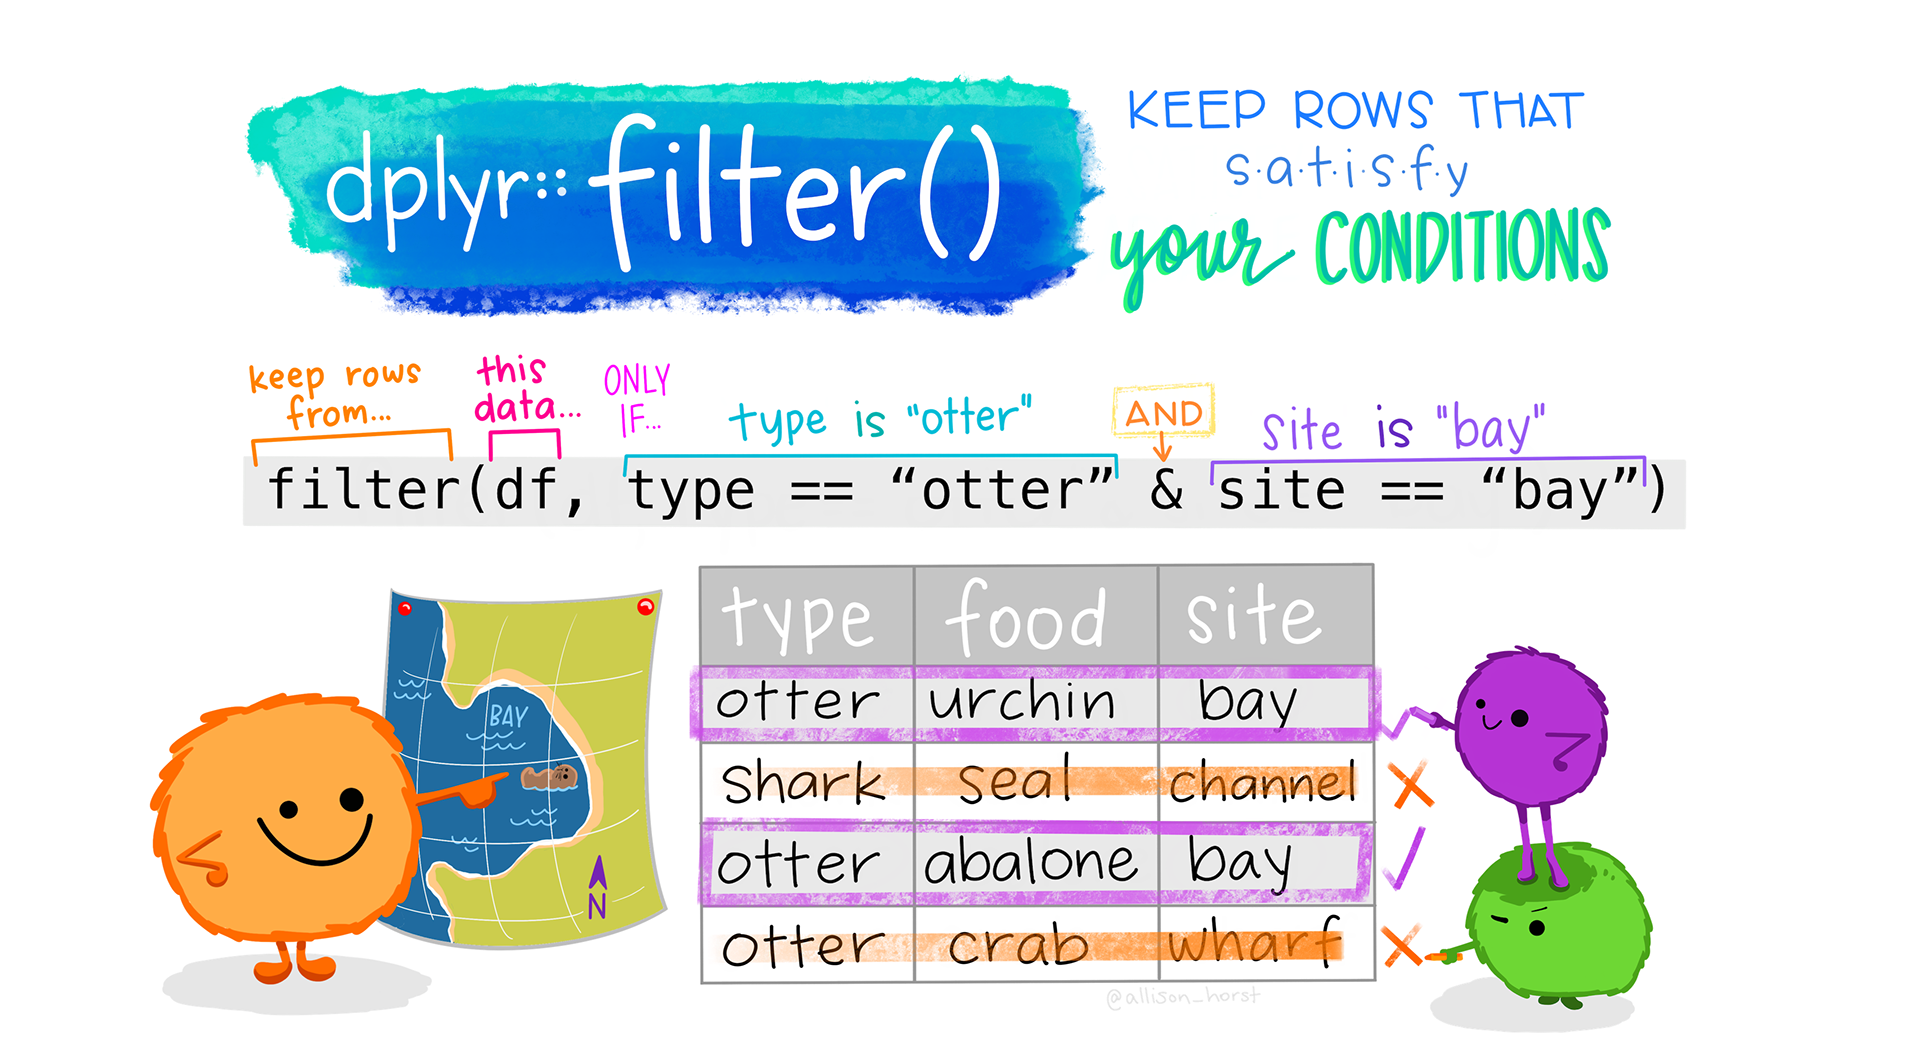
\includegraphics[width=0.8\textwidth,height=\textheight]{118_B_wrangling_files/mediabag/cb8d9c50-f48e-4c6d-a.png}

}

\caption{Artwork by @allisonhorst}

\end{figure}

For example, we may be interested in only looking at only the languages
in this dataset that are Aboriginal languages.

Start with the \texttt{can\_lang\ dataset}, the pipe
``\%\textgreater\%'' means apply the action on the following line to the
previous line.

\hypertarget{annotated-cell-5}{%
\label{annotated-cell-5}}%
\begin{Shaded}
\begin{Highlighting}[]
\NormalTok{can\_lang  }\SpecialCharTok{\%\textgreater{}\%}                                  \CommentTok{\#\textless{}1\textgreater{}}
  \FunctionTok{filter}\NormalTok{(category }\SpecialCharTok{==} \StringTok{"Aboriginal languages"}\NormalTok{)   }\CommentTok{\#\textless{}2\textgreater{}}
\end{Highlighting}
\end{Shaded}

\begin{description}
\tightlist
\item[\circled{1}]
begin with the \texttt{can\_lang} dataset
\item[\circled{2}]
only include the rows were the category variable is ``Aboriginal
languages''
\end{description}

\begin{verbatim}
               category                     language mother_tongue most_at_home
1  Aboriginal languages Aboriginal languages, n.o.s.           590          235
2  Aboriginal languages Algonquian languages, n.i.e.            45           10
3  Aboriginal languages                    Algonquin          1260          370
4  Aboriginal languages Athabaskan languages, n.i.e.            50           10
5  Aboriginal languages                    Atikamekw          6150         5465
6  Aboriginal languages         Babine (Wetsuwet'en)           110           20
7  Aboriginal languages                       Beaver           190           50
8  Aboriginal languages                    Blackfoot          2815         1110
9  Aboriginal languages                      Carrier          1025          250
10 Aboriginal languages                       Cayuga            45           10
11 Aboriginal languages                    Chilcotin           655          255
12 Aboriginal languages                        Comox            85            0
13 Aboriginal languages                 Cree, n.o.s.         64050        37950
14 Aboriginal languages                       Dakota          1210          255
15 Aboriginal languages                         Dene         10700         7710
16 Aboriginal languages              Dogrib (Tlicho)          1650         1020
17 Aboriginal languages            Gitxsan (Gitksan)           880          315
18 Aboriginal languages                     Gwich'in           255           50
19 Aboriginal languages                        Haida            80           10
20 Aboriginal languages                       Haisla            90           20
21 Aboriginal languages                   Halkomelem           480           50
22 Aboriginal languages                     Heiltsuk           100            5
23 Aboriginal languages   Inuinnaqtun (Inuvialuktun)          1020          165
24 Aboriginal languages      Inuit languages, n.i.e.           310           90
25 Aboriginal languages                    Inuktitut         35210        29230
26 Aboriginal languages  Iroquoian languages, n.i.e.            35            5
27 Aboriginal languages               Kaska (Nahani)           180           20
28 Aboriginal languages                      Kutenai           110           10
29 Aboriginal languages         Kwakiutl (Kwak'wala)           325           25
30 Aboriginal languages                     Lillooet           315           25
31 Aboriginal languages                     Malecite           300           55
32 Aboriginal languages                      Mi'kmaq          6690         3565
33 Aboriginal languages                       Michif           465           80
34 Aboriginal languages                       Mohawk           985          255
35 Aboriginal languages            Montagnais (Innu)         10235         8585
36 Aboriginal languages                   Moose Cree           105           10
37 Aboriginal languages                      Naskapi          1205         1195
38 Aboriginal languages                      Nisga'a           400           75
39 Aboriginal languages          North Slavey (Hare)           765          340
40 Aboriginal languages           Northern East Cree           315          110
41 Aboriginal languages            Northern Tutchone           220           30
42 Aboriginal languages      Nuu-chah-nulth (Nootka)           280           30
43 Aboriginal languages                     Oji-Cree         12855         7905
44 Aboriginal languages                      Ojibway         17885         6175
45 Aboriginal languages                     Okanagan           275           80
46 Aboriginal languages                       Oneida            60           15
47 Aboriginal languages               Ottawa (Odawa)           150           75
48 Aboriginal languages                  Plains Cree          3065         1345
49 Aboriginal languages     Salish languages, n.i.e.           260           25
50 Aboriginal languages               Sarsi (Sarcee)            80           10
51 Aboriginal languages                       Sekani            85           15
52 Aboriginal languages      Shuswap (Secwepemctsin)           445           50
53 Aboriginal languages     Siouan languages, n.i.e.            55           20
54 Aboriginal languages               Slavey, n.o.s.           280          105
55 Aboriginal languages                 South Slavey           945          370
56 Aboriginal languages           Southern East Cree            45           15
57 Aboriginal languages            Southern Tutchone            70            5
58 Aboriginal languages                     Squamish            40            5
59 Aboriginal languages                       Stoney          3025         1950
60 Aboriginal languages                      Straits            80           25
61 Aboriginal languages                  Swampy Cree          1440          330
62 Aboriginal languages                      Tahltan            95            5
63 Aboriginal languages       Thompson (Ntlakapamux)           335           20
64 Aboriginal languages                      Tlingit            95            0
65 Aboriginal languages                    Tsimshian           200           30
66 Aboriginal languages   Wakashan languages, n.i.e.            10            0
67 Aboriginal languages                   Woods Cree          1840          800
   most_at_work lang_known
1            30        665
2             0        120
3            40       2480
4             0         85
5          1100       6645
6            10        210
7             0        340
8            85       5645
9            15       2100
10           10        125
11           15       1150
12            0        185
13         7800      86115
14           20       1760
15          770      13060
16          165       2375
17           10       1305
18           10        360
19            0        465
20            0        175
21           20       1060
22           10        125
23           30       1975
24           15        470
25         8795      40620
26            0        115
27           10        365
28            0        170
29           15        605
30           15        790
31           10        760
32          915       9025
33           10       1210
34           30       2415
35         2055      11445
36            0        195
37          370       1465
38           10       1055
39           95       1005
40           35        550
41            0        280
42           10        560
43         1080      15605
44          765      28580
45           20        820
46            0        185
47            0        205
48           95       5905
49            0        560
50            0        145
51            0        185
52           35       1305
53            0        140
54           10        675
55           35       1365
56            0         40
57            0        145
58           10        285
59          240       3675
60           15        365
61           10       2350
62            0        265
63            0        450
64           10        260
65           10        410
66            0         25
67           75       2665
\end{verbatim}

Some notes:

\begin{itemize}
\tightlist
\item
  the aboriginal languages is text/categorical and so quotation marks
  are needed.
\item
  R doesn't care about whether they are double quotation marks (``) or
  single ('). They work the same.
\item
  If we don't assign it to an object, then it just prints out for us to
  see!
\end{itemize}

Oftentimes, we want to take our subset and give it a new name. This
takes our subset and assigns it to a new dataset called
\texttt{aboriginal\_lang}.

\hypertarget{annotated-cell-6}{%
\label{annotated-cell-6}}%
\begin{Shaded}
\begin{Highlighting}[]
\NormalTok{aboriginal\_lang }\OtherTok{\textless{}{-}}\NormalTok{ can\_lang  }\SpecialCharTok{\%\textgreater{}\%}             \CommentTok{\#\textless{}1\textgreater{} }
  \FunctionTok{filter}\NormalTok{(category }\SpecialCharTok{==} \StringTok{"Aboriginal languages"}\NormalTok{)  }
\end{Highlighting}
\end{Shaded}

\begin{description}
\tightlist
\item[\circled{1}]
The code \texttt{aboriginal\_lang\ \textless{}-} takes the given data
(the Aboriginal languages in the \texttt{can\_lang} dataset) and saves
it as a new object called \texttt{aboriginal\_lang}.
\end{description}

Notes:

\begin{itemize}
\tightlist
\item
  Notice if you assign it to an object that it doesn't print out the
  contents.
\item
  You'll see the new object in your environment on the top right
  ---\textgreater{}
\end{itemize}

It can also be used with numeric criteria.

Suppose we want a list of all the languages in Canada that are spoken by
less than 100 people as their mother tongue.

\hypertarget{annotated-cell-7}{%
\label{annotated-cell-7}}%
\begin{Shaded}
\begin{Highlighting}[]
\NormalTok{rare\_lang }\OtherTok{\textless{}{-}}\NormalTok{ can\_lang  }\SpecialCharTok{\%\textgreater{}\%}        \CommentTok{\#\textless{}1\textgreater{}     }
  \FunctionTok{filter}\NormalTok{(mother\_tongue }\SpecialCharTok{\textless{}} \DecValTok{100}\NormalTok{)     }\CommentTok{\#\textless{}2\textgreater{}}
                                  \CommentTok{\#\textless{}3\textgreater{}}
\end{Highlighting}
\end{Shaded}

\begin{description}
\tightlist
\item[\circled{1}]
begin with the \texttt{can\_lang} dataset
\item[\circled{2}]
only include the rows were the number of people who speak the language
as their mother tongue is more than 100 people
\item[\circled{3}]
data saved to the object \texttt{rare\_lang}
\end{description}

The logical operators are given below:

\begin{longtable}[]{@{}ll@{}}
\toprule\noalign{}
Operator & Description \\
\midrule\noalign{}
\endhead
\bottomrule\noalign{}
\endlastfoot
\texttt{\textless{}} & Less than \\
\texttt{\textgreater{}} & Greater than \\
\texttt{\textless{}=} & Less than or equal to \\
\texttt{\textgreater{}=} & Greater than or equal to \\
\texttt{==} & Equal to \\
\texttt{!=} & Not equal to \\
\texttt{!x} & Not x \\
\texttt{x\ \textbar{}\ y} & x OR y \\
\texttt{x\ \&\ y} & x AND y \\
\end{longtable}

\hypertarget{select}{%
\section{\texorpdfstring{\texttt{select}}{select}}\label{select}}

\texttt{select} is used to extract only certain \textbf{\emph{columns}}.
For example, perhaps we only want to print out a list names of the
aboriginal languages (language column).

\hypertarget{annotated-cell-8}{%
\label{annotated-cell-8}}%
\begin{Shaded}
\begin{Highlighting}[]
\NormalTok{aboriginal\_lang }\SpecialCharTok{\%\textgreater{}\%}  \CommentTok{\#\textless{}1\textgreater{}}
  \FunctionTok{select}\NormalTok{(language)  }\CommentTok{\#\textless{}2\textgreater{}}
\end{Highlighting}
\end{Shaded}

\begin{description}
\tightlist
\item[\circled{1}]
Begin with the \texttt{aboriginal\_lang} dataset
\item[\circled{2}]
only include the language column
\end{description}

\begin{verbatim}
                       language
1  Aboriginal languages, n.o.s.
2  Algonquian languages, n.i.e.
3                     Algonquin
4  Athabaskan languages, n.i.e.
5                     Atikamekw
6          Babine (Wetsuwet'en)
7                        Beaver
8                     Blackfoot
9                       Carrier
10                       Cayuga
11                    Chilcotin
12                        Comox
13                 Cree, n.o.s.
14                       Dakota
15                         Dene
16              Dogrib (Tlicho)
17            Gitxsan (Gitksan)
18                     Gwich'in
19                        Haida
20                       Haisla
21                   Halkomelem
22                     Heiltsuk
23   Inuinnaqtun (Inuvialuktun)
24      Inuit languages, n.i.e.
25                    Inuktitut
26  Iroquoian languages, n.i.e.
27               Kaska (Nahani)
28                      Kutenai
29         Kwakiutl (Kwak'wala)
30                     Lillooet
31                     Malecite
32                      Mi'kmaq
33                       Michif
34                       Mohawk
35            Montagnais (Innu)
36                   Moose Cree
37                      Naskapi
38                      Nisga'a
39          North Slavey (Hare)
40           Northern East Cree
41            Northern Tutchone
42      Nuu-chah-nulth (Nootka)
43                     Oji-Cree
44                      Ojibway
45                     Okanagan
46                       Oneida
47               Ottawa (Odawa)
48                  Plains Cree
49     Salish languages, n.i.e.
50               Sarsi (Sarcee)
51                       Sekani
52      Shuswap (Secwepemctsin)
53     Siouan languages, n.i.e.
54               Slavey, n.o.s.
55                 South Slavey
56           Southern East Cree
57            Southern Tutchone
58                     Squamish
59                       Stoney
60                      Straits
61                  Swampy Cree
62                      Tahltan
63       Thompson (Ntlakapamux)
64                      Tlingit
65                    Tsimshian
66   Wakashan languages, n.i.e.
67                   Woods Cree
\end{verbatim}

We can combine criteria together as well in one command with multiple
pipes:

\begin{Shaded}
\begin{Highlighting}[]
\NormalTok{can\_lang }\SpecialCharTok{\%\textgreater{}\%} 
  \FunctionTok{filter}\NormalTok{(category }\SpecialCharTok{==} \StringTok{"Aboriginal languages"}\NormalTok{) }\SpecialCharTok{\%\textgreater{}\%} 
  \FunctionTok{select}\NormalTok{(language)}
\end{Highlighting}
\end{Shaded}

\begin{verbatim}
                       language
1  Aboriginal languages, n.o.s.
2  Algonquian languages, n.i.e.
3                     Algonquin
4  Athabaskan languages, n.i.e.
5                     Atikamekw
6          Babine (Wetsuwet'en)
7                        Beaver
8                     Blackfoot
9                       Carrier
10                       Cayuga
11                    Chilcotin
12                        Comox
13                 Cree, n.o.s.
14                       Dakota
15                         Dene
16              Dogrib (Tlicho)
17            Gitxsan (Gitksan)
18                     Gwich'in
19                        Haida
20                       Haisla
21                   Halkomelem
22                     Heiltsuk
23   Inuinnaqtun (Inuvialuktun)
24      Inuit languages, n.i.e.
25                    Inuktitut
26  Iroquoian languages, n.i.e.
27               Kaska (Nahani)
28                      Kutenai
29         Kwakiutl (Kwak'wala)
30                     Lillooet
31                     Malecite
32                      Mi'kmaq
33                       Michif
34                       Mohawk
35            Montagnais (Innu)
36                   Moose Cree
37                      Naskapi
38                      Nisga'a
39          North Slavey (Hare)
40           Northern East Cree
41            Northern Tutchone
42      Nuu-chah-nulth (Nootka)
43                     Oji-Cree
44                      Ojibway
45                     Okanagan
46                       Oneida
47               Ottawa (Odawa)
48                  Plains Cree
49     Salish languages, n.i.e.
50               Sarsi (Sarcee)
51                       Sekani
52      Shuswap (Secwepemctsin)
53     Siouan languages, n.i.e.
54               Slavey, n.o.s.
55                 South Slavey
56           Southern East Cree
57            Southern Tutchone
58                     Squamish
59                       Stoney
60                      Straits
61                  Swampy Cree
62                      Tahltan
63       Thompson (Ntlakapamux)
64                      Tlingit
65                    Tsimshian
66   Wakashan languages, n.i.e.
67                   Woods Cree
\end{verbatim}

\hypertarget{arrange}{%
\section{\texorpdfstring{\texttt{arrange}}{arrange}}\label{arrange}}

The \texttt{arrange} function allows us to order the rows of the data
frame by the values of a particular column.

For example, arrange all the aboriginal languages in canada by from most
to least spoken as mother tongue.

\hypertarget{annotated-cell-10}{%
\label{annotated-cell-10}}%
\begin{Shaded}
\begin{Highlighting}[]
\NormalTok{aboriginal\_lang }\SpecialCharTok{\%\textgreater{}\%} 
  \FunctionTok{arrange}\NormalTok{(}\FunctionTok{desc}\NormalTok{(mother\_tongue))  }\CommentTok{\#\textless{}1\textgreater{}}
\end{Highlighting}
\end{Shaded}

\begin{description}
\tightlist
\item[\circled{1}]
arranges the languages from the language with the most to the least
people who speak the language as their mother tongue
\end{description}

\begin{verbatim}
               category                     language mother_tongue most_at_home
1  Aboriginal languages                 Cree, n.o.s.         64050        37950
2  Aboriginal languages                    Inuktitut         35210        29230
3  Aboriginal languages                      Ojibway         17885         6175
4  Aboriginal languages                     Oji-Cree         12855         7905
5  Aboriginal languages                         Dene         10700         7710
6  Aboriginal languages            Montagnais (Innu)         10235         8585
7  Aboriginal languages                      Mi'kmaq          6690         3565
8  Aboriginal languages                    Atikamekw          6150         5465
9  Aboriginal languages                  Plains Cree          3065         1345
10 Aboriginal languages                       Stoney          3025         1950
11 Aboriginal languages                    Blackfoot          2815         1110
12 Aboriginal languages                   Woods Cree          1840          800
13 Aboriginal languages              Dogrib (Tlicho)          1650         1020
14 Aboriginal languages                  Swampy Cree          1440          330
15 Aboriginal languages                    Algonquin          1260          370
16 Aboriginal languages                       Dakota          1210          255
17 Aboriginal languages                      Naskapi          1205         1195
18 Aboriginal languages                      Carrier          1025          250
19 Aboriginal languages   Inuinnaqtun (Inuvialuktun)          1020          165
20 Aboriginal languages                       Mohawk           985          255
21 Aboriginal languages                 South Slavey           945          370
22 Aboriginal languages            Gitxsan (Gitksan)           880          315
23 Aboriginal languages          North Slavey (Hare)           765          340
24 Aboriginal languages                    Chilcotin           655          255
25 Aboriginal languages Aboriginal languages, n.o.s.           590          235
26 Aboriginal languages                   Halkomelem           480           50
27 Aboriginal languages                       Michif           465           80
28 Aboriginal languages      Shuswap (Secwepemctsin)           445           50
29 Aboriginal languages                      Nisga'a           400           75
30 Aboriginal languages       Thompson (Ntlakapamux)           335           20
31 Aboriginal languages         Kwakiutl (Kwak'wala)           325           25
32 Aboriginal languages                     Lillooet           315           25
33 Aboriginal languages           Northern East Cree           315          110
34 Aboriginal languages      Inuit languages, n.i.e.           310           90
35 Aboriginal languages                     Malecite           300           55
36 Aboriginal languages      Nuu-chah-nulth (Nootka)           280           30
37 Aboriginal languages               Slavey, n.o.s.           280          105
38 Aboriginal languages                     Okanagan           275           80
39 Aboriginal languages     Salish languages, n.i.e.           260           25
40 Aboriginal languages                     Gwich'in           255           50
41 Aboriginal languages            Northern Tutchone           220           30
42 Aboriginal languages                    Tsimshian           200           30
43 Aboriginal languages                       Beaver           190           50
44 Aboriginal languages               Kaska (Nahani)           180           20
45 Aboriginal languages               Ottawa (Odawa)           150           75
46 Aboriginal languages         Babine (Wetsuwet'en)           110           20
47 Aboriginal languages                      Kutenai           110           10
48 Aboriginal languages                   Moose Cree           105           10
49 Aboriginal languages                     Heiltsuk           100            5
50 Aboriginal languages                      Tahltan            95            5
51 Aboriginal languages                      Tlingit            95            0
52 Aboriginal languages                       Haisla            90           20
53 Aboriginal languages                        Comox            85            0
54 Aboriginal languages                       Sekani            85           15
55 Aboriginal languages                        Haida            80           10
56 Aboriginal languages               Sarsi (Sarcee)            80           10
57 Aboriginal languages                      Straits            80           25
58 Aboriginal languages            Southern Tutchone            70            5
59 Aboriginal languages                       Oneida            60           15
60 Aboriginal languages     Siouan languages, n.i.e.            55           20
61 Aboriginal languages Athabaskan languages, n.i.e.            50           10
62 Aboriginal languages Algonquian languages, n.i.e.            45           10
63 Aboriginal languages                       Cayuga            45           10
64 Aboriginal languages           Southern East Cree            45           15
65 Aboriginal languages                     Squamish            40            5
66 Aboriginal languages  Iroquoian languages, n.i.e.            35            5
67 Aboriginal languages   Wakashan languages, n.i.e.            10            0
   most_at_work lang_known
1          7800      86115
2          8795      40620
3           765      28580
4          1080      15605
5           770      13060
6          2055      11445
7           915       9025
8          1100       6645
9            95       5905
10          240       3675
11           85       5645
12           75       2665
13          165       2375
14           10       2350
15           40       2480
16           20       1760
17          370       1465
18           15       2100
19           30       1975
20           30       2415
21           35       1365
22           10       1305
23           95       1005
24           15       1150
25           30        665
26           20       1060
27           10       1210
28           35       1305
29           10       1055
30            0        450
31           15        605
32           15        790
33           35        550
34           15        470
35           10        760
36           10        560
37           10        675
38           20        820
39            0        560
40           10        360
41            0        280
42           10        410
43            0        340
44           10        365
45            0        205
46           10        210
47            0        170
48            0        195
49           10        125
50            0        265
51           10        260
52            0        175
53            0        185
54            0        185
55            0        465
56            0        145
57           15        365
58            0        145
59            0        185
60            0        140
61            0         85
62            0        120
63           10        125
64            0         40
65           10        285
66            0        115
67            0         25
\end{verbatim}

Note:

\begin{itemize}
\tightlist
\item
  use arrange(variable) to go from least to most
\item
  use arrange(desc(variable)) to go from most to least,
  arrange(-variable) also works
\end{itemize}

\hypertarget{slice}{%
\section{\texorpdfstring{\texttt{slice}}{slice}}\label{slice}}

The slice function will allow us to pick only a subset of the rows based
on their numeric order (1st through last).

For example, if I want a list of the 10 most commonly spoken aboriginal
languages.

\hypertarget{annotated-cell-11}{%
\label{annotated-cell-11}}%
\begin{Shaded}
\begin{Highlighting}[]
\NormalTok{aboriginal\_lang }\SpecialCharTok{\%\textgreater{}\%} 
  \FunctionTok{arrange}\NormalTok{(}\FunctionTok{desc}\NormalTok{(mother\_tongue)) }\SpecialCharTok{\%\textgreater{}\%} 
  \FunctionTok{slice}\NormalTok{(}\DecValTok{1}\SpecialCharTok{:}\DecValTok{10}\NormalTok{)   }\CommentTok{\#\textless{}1\textgreater{}}
\end{Highlighting}
\end{Shaded}

\begin{description}
\tightlist
\item[\circled{1}]
Only include the first 10 rows of the dataset
\end{description}

\begin{verbatim}
               category          language mother_tongue most_at_home
1  Aboriginal languages      Cree, n.o.s.         64050        37950
2  Aboriginal languages         Inuktitut         35210        29230
3  Aboriginal languages           Ojibway         17885         6175
4  Aboriginal languages          Oji-Cree         12855         7905
5  Aboriginal languages              Dene         10700         7710
6  Aboriginal languages Montagnais (Innu)         10235         8585
7  Aboriginal languages           Mi'kmaq          6690         3565
8  Aboriginal languages         Atikamekw          6150         5465
9  Aboriginal languages       Plains Cree          3065         1345
10 Aboriginal languages            Stoney          3025         1950
   most_at_work lang_known
1          7800      86115
2          8795      40620
3           765      28580
4          1080      15605
5           770      13060
6          2055      11445
7           915       9025
8          1100       6645
9            95       5905
10          240       3675
\end{verbatim}

\hypertarget{mutate}{%
\section{\texorpdfstring{\texttt{mutate}}{mutate}}\label{mutate}}

\texttt{mutate()} creates new columns that are functions of existing
variables.

\begin{figure}

{\centering 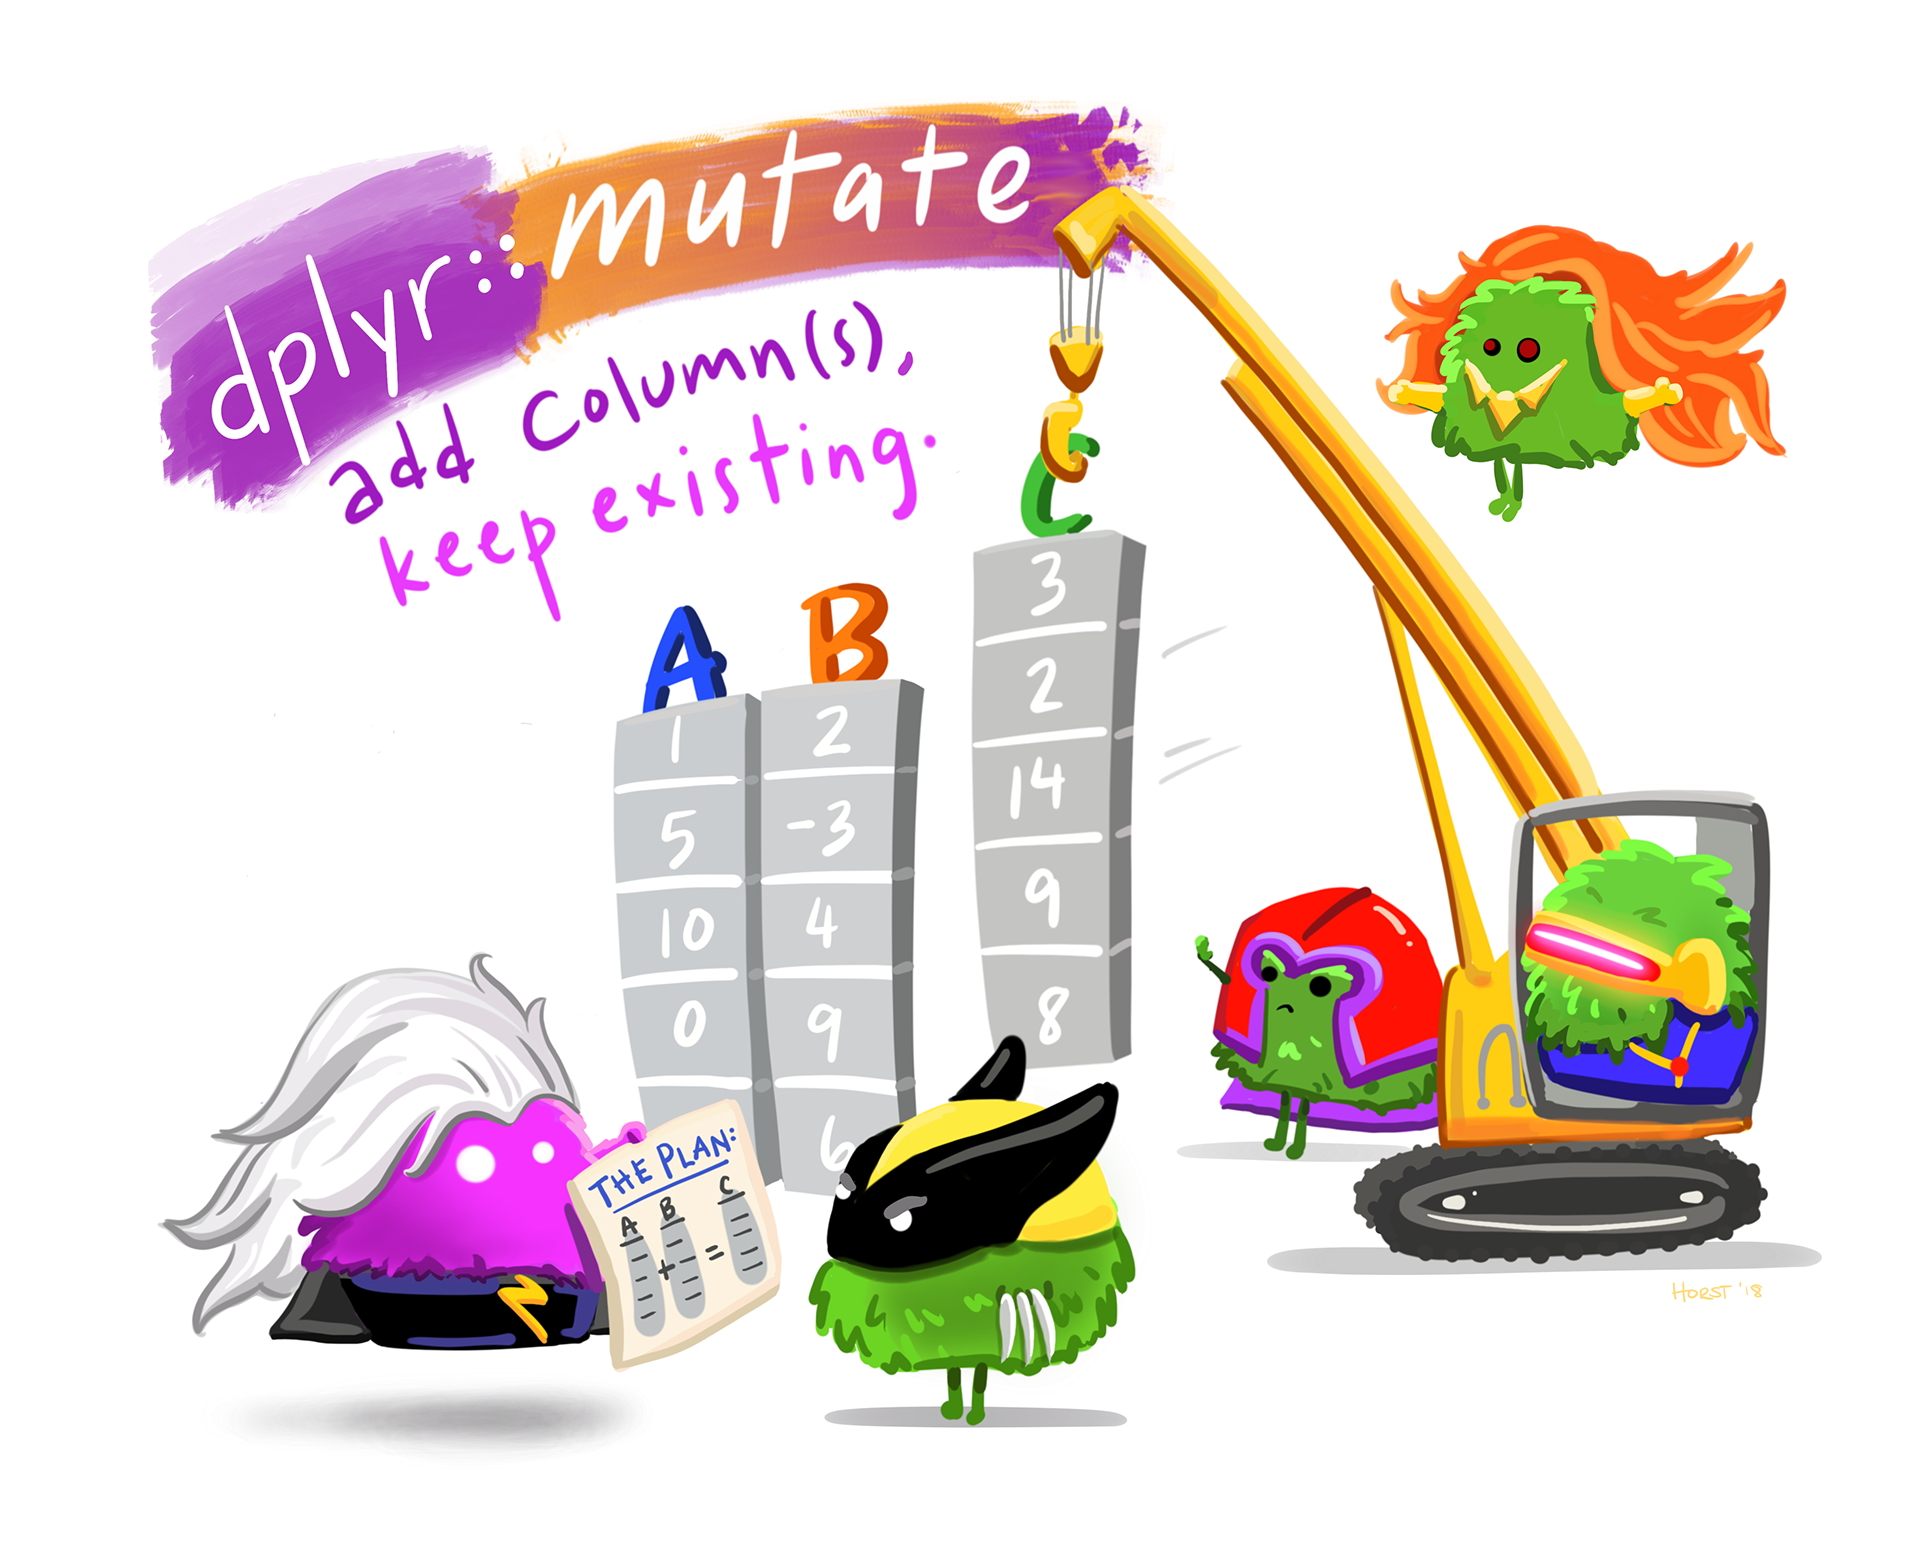
\includegraphics{118_B_wrangling_files/mediabag/bd4ae264-ae51-4d18-b.png}

}

\caption{Artwork by @allisonhorst}

\end{figure}

For example, if I want to create a new column called
\texttt{mother\_tongue\_K} which represents the number of people who
speak the language their mother tongue in thousands. You may want to
save this new dataset over top of the original dataset so you could use
this new column in the future.

\hypertarget{annotated-cell-12}{%
\label{annotated-cell-12}}%
\begin{Shaded}
\begin{Highlighting}[]
\NormalTok{aboriginal\_lang }\OtherTok{\textless{}{-}}\NormalTok{ aboriginal\_lang }\SpecialCharTok{\%\textgreater{}\%} 
  \FunctionTok{mutate}\NormalTok{(}\AttributeTok{mother\_tongue\_K =}\NormalTok{ mother\_tongue}\SpecialCharTok{/}\DecValTok{1000}\NormalTok{) }\CommentTok{\#\textless{}1\textgreater{}}
\end{Highlighting}
\end{Shaded}

\begin{description}
\tightlist
\item[\circled{1}]
Creates a new column called \texttt{mother\_tongue\_K} calculated by
taking the \texttt{mother\_tongue} column and dividing it by 1000.
\end{description}

This can be useful for unit conversions. It also be useful for making
new calculations based on existing data (for example, price and number
of square feet could be used to calculate price per square foot).



\end{document}
